\documentclass{article}
\usepackage{graphicx} % Required for inserting images
\usepackage[italian]{babel}
\usepackage[T1]{fontenc}
\usepackage{microtype}
\usepackage{lmodern}
\usepackage{amsmath}
\usepackage{float}
\usepackage{caption}
\usepackage{amssymb}
\usepackage{hyperref}
\emergencystretch=2em
\setlength{\parindent}{0pt}

\title{Documentazione - Deck-BuilderCR}
\author{Vito Francesco Maistrini - Giovanni De Caro - Mauro Gorga}
\date{Gennaio 2026}

\begin{document}

\maketitle
\begin{figure}[h]
\centering

\includegraphics[width=0.25\textwidth]{images/logo.png}
\end{figure}
\tableofcontents

\section{Definizione del problema}
\subsection{Introduzione}
Il progetto Deck-BuilderCR nasce per ovviare al problema della costruzione di un deck in Clash Royale
che consiste nel selezionare un insieme limitato di carte (8), a partire da un insieme molto ampio di possibilità (truppe/edifici/incantesimi), dove ognuna ha un proprio costo di elisir (che varia dall’1 al 9).\\
La complessità del problema deriva dal fatto che lo spazio delle possibili combinazioni cresce in maniera combinatoria all’aumentare del numero di carte presenti nel gioco, e che la qualità del deck non dipende solo dalle singole carte, ma:
\begin{itemize}
  \item Dall’efficienza della combinazione tra le carte 
  \item Dal costo medio dell’elisir del deck 
  \item Dalla Diversificazione della tipologia delle carte (truppe/edifici/incantesimi)
\end{itemize}
Dunque, il progetto Deck-BuilderCR è stato pensato principalmente per rivolgersi a dei giocatori alle prime armi e aiutarli a costruire deck bilanciati sotto tutti i vari punti di vista del gioco; questo dato che le carte presenti nel gioco sono tante e le combinazioni possibili per un deck raggiungono un numero spropositato.


\subsection{Obiettivi}
L’obiettivo principale del progetto Deck-BuilderCR, è la creazione di un sistema di IA in grado di generare automaticamente deck ottimizzati per Clash Royale, rispettando vincoli strutturali imposti dall’utente e massimizzando una misura di qualità del deck in base a dei vincoli interni del programma.
In particolare, il sistema deve:

\begin{itemize}
  \item Generare deck composti esattamente da 8 carte 
  \item Garantire la coerenza del deck con dei vincoli selezionati dall’utente (tra quelli disponibili)
  \item Rispettare vincoli imposti dal gioco e dal sistema
  \item Massimizzare una funzione di valutazione che tenga conto della qualità complessiva del deck 
  \item Fornire un output comprensibile all’utente finale tramite una dashboard che mostri il deck generato e ne spieghi le caratteristiche principali
\end{itemize}

\subsection{Specifica PEAS}

La specifica PEAS (Performance, Environment, Actuators, Sensors) viene utilizzata per descrivere formalmente il contesto operativo dell’agente.

\paragraph{Performance (misure di prestazione:)}
Le metriche utilizzate per valutare l’operato dell’agente sono:
\begin{itemize}
    \item Qualità complessiva del deck generato, misurata tramite una funzione di fitness multi-criterio soggetta a vincoli.
    \item Rispetto dei vincoli imposti, quali costo medio in elisir, carte fissate dall’utente, bilanciamento dei ruoli e tipologia delle truppe.
    \item Tempo di esecuzione e risorse computazionali utilizzate dall’algoritmo.
\end{itemize}

\paragraph{Environment (ambiente):}
L’ambiente in cui opera l’agente è costituito da:
\begin{itemize}
    \item L’insieme delle carte disponibili con le rispettive caratteristiche.
    \item Le regole di composizione di un deck, che prevedono un numero fisso di 8 carte.
\end{itemize}

\paragraph{Actuators (attuatori):}
Le azioni che l’agente può intraprendere sono:
\begin{itemize}
    \item Selezione di una carta da includere nel deck.
    \item Sostituzione di una carta con un’altra carta disponibile.
\end{itemize}

\paragraph{Sensors (sensori):}
Le informazioni percettive disponibili all’agente sono:
\begin{itemize}
    \item Caratteristiche delle singole carte (costo, ruolo, tipologia, statistiche).
    \item Costo medio in elisir del deck.
    \item Copertura dei ruoli fondamentali nel deck.
    \item Valore della funzione di valutazione associata al deck corrente.
\end{itemize}

\subsubsection{Caratteristiche dell’ambiente}

Il problema può essere classificato secondo le seguenti proprietà dell’ambiente:

\paragraph{Singolo agente:}
Il problema è modellato come un problema a singolo agente, in cui non sono presenti altri agenti o avversari espliciti durante il processo di ricerca.

\paragraph{Completamente osservabile:}
L’ambiente è completamente osservabile, poiché l’agente ha accesso a tutte le informazioni rilevanti sulle carte disponibili, sui vincoli di composizione del deck e sul valore della funzione di valutazione.

\paragraph{Deterministico:}
L’ambiente è deterministico: a una data configurazione del deck e a una specifica azione (ad esempio la sostituzione di una carta) corrisponde sempre lo stesso stato successivo.

\paragraph{Sequenziale:}
Il processo di ricerca è sequenziale e consiste in una serie di trasformazioni dello stato finalizzate al miglioramento progressivo della soluzione. Le decisioni prese influenzano gli stati futuri.

\paragraph{Statico:}
L’ambiente è statico durante l’esecuzione dell’algoritmo, poiché le caratteristiche delle carte e i vincoli di composizione non variano nel tempo.

\paragraph{Discreto:}
Lo spazio degli stati è discreto, in quanto ogni deck è composto da un numero finito di carte selezionate da un insieme discreto.

\subsection{Analisi del problema:}

Il problema può essere formalizzato come un problema di ricerca in uno spazio degli stati, in cui ogni stato rappresenta un possibile deck valido o parzialmente valido.

\paragraph{Stati:}
Ogni stato rappresenta una configurazione di deck composta da un sottoinsieme di 8 carte.

\paragraph{Stato iniziale:}
Lo stato iniziale è un deck generato casualmente oppure un deck parzialmente definito dall’utente, il quale può fissare una o più carte.

\paragraph{Azioni:}
L’agente può eseguire due tipologie di azioni:
\begin{itemize}
    \item Aggiunta di una carta al deck.
    \item Sostituzione di una carta con un’altra carta disponibile.
\end{itemize}

\paragraph{Spazio degli stati:}
Lo spazio degli stati è costituito da tutte le possibili combinazioni di 8 carte selezionabili dall’insieme totale delle carte disponibili.

\paragraph{Test obiettivo:}
L’obiettivo è la massimizzazione della qualità del deck secondo una funzione di valutazione (fitness function).\\


Il problema presenta le seguenti caratteristiche:
\begin{itemize}
    \item Spazio degli stati estremamente ampio.
    \item Assenza di una soluzione ottima facilmente calcolabile in modo esatto.
    \item Presenza di molteplici vincoli da soddisfare simultaneamente.
    \item Necessità di bilanciare la qualità della soluzione con il costo computazionale.
\end{itemize}

A dicembre 2025 Clash Royale mette a disposizione 121 carte, per un numero di deck possibili pari a $899{,}749{,}479{,}915$.
Pertanto il problema non è risolvibile tramite ricerca esaustiva ed è più adatto all’impiego di tecniche di ricerca approssimata e ottimizzazione, come gli algoritmi genetici, che consentono di esplorare efficacemente lo spazio delle soluzioni senza enumerarlo completamente.

\subsection{Assunzioni e limitazioni del dominio}

Per il progetto \textit{Deck-BuilderCR}, il dominio del problema è stato intenzionalmente semplificato introducendo alcune assunzioni e limitazioni, al fine di rendere il problema trattabile e di concentrarsi sugli aspetti di ricerca e ottimizzazione.

In particolare, non sono state prese in considerazione le evoluzioni delle carte, i campioni e gli eroi (introdotti recentemente nel gioco). 
Tali elementi presentano meccaniche avanzate e dinamiche di gioco complesse, che richiederebbero un modello di valutazione più articolato e una rappresentazione dello stato significativamente più estesa. 
Di conseguenza, il numero totale di carte considerate nel dominio è pari a 113.

L’esclusione di queste componenti consente di:
\begin{itemize}
    \item Ridurre la dimensionalità dello spazio degli stati.
    \item Focalizzare l’analisi sull’efficacia degli algoritmi di ricerca adottati.
\end{itemize}

\subsection{Caratteristiche del gioco}

\subsubsection{Caratteristiche delle carte}

Una carta rappresenta un componente elementare della soluzione (deck). 
Ogni carta è descritta mediante i seguenti attributi:

\begin{itemize}
    \item \textbf{Danno/s}: danno inflitto al secondo.
    \item \textbf{Punti vita}: danni necessari per eliminare la carta.
    \item \textbf{Costo}: costo in elisir per schierare la carta.
    \item \textbf{Volante}: valore booleano che indica se la truppa non può essere colpita da unità da mischia.
    \item \textbf{Tipologia}: truppa, incantesimo o edificio.
    \item \textbf{Velocità}: velocità di movimento discretizzata (\textit{lento}=0, \textit{medio}=1, \textit{rapido}=2, \textit{molto rapido}=3).
    \item \textbf{Portata}: valore booleano, pari a 1 se la carta colpisce unità terrestri e volanti, 0 se colpisce solo unità terrestri.
    \item \textbf{Tipo di bersaglio}: valore booleano, pari a 1 se il bersaglio è esclusivamente la torre, 0 se il bersaglio include sia truppe sia torri.
    \item \textbf{Effetti aggiuntivi}: valore numerico intero che rappresenta la potenza degli effetti speciali della carta, compreso tra 0 e 2 (ad esempio congelamento, rallentamento, generazione di truppe, danni ad area, scudi).
\end{itemize}

La valutazione è un’euristica empirica utilizzata per stimare in modo approssimato il contributo strategico della carta.
Il valore assegnato agli effetti aggiuntivi è in parte soggettivo e dipende dall’esperienza di gioco.

\subsubsection{Caratteristiche degli stati}

Uno stato è rappresentato da una configurazione di 8 carte (deck). 
Ogni deck è descritto dai seguenti attributi aggregati:

\begin{itemize}
    \item \textbf{Danno medio/s}: media aritmetica del danno al secondo delle carte.
    \item \textbf{Punti ferita medi}: media aritmetica dei punti vita delle carte (escludendo gli incantesimi).
    \item \textbf{Costo medio}: media aritmetica del costo in elisir delle carte.
    \item \textbf{Numero di truppe volanti}: numero di carte di tipo truppa volante.
    \item \textbf{Numero di edifici}: numero di carte di tipologia edificio.
    \item \textbf{Numero di incantesimi}: numero di carte di tipologia incantesimo.
    \item \textbf{Velocità media}: media aritmetica della velocità delle carte.
    \item \textbf{Numero di carte con portata}: numero di carte che colpiscono unità terrestri e volanti.
    \item \textbf{Numero di carte con bersaglio torre}: numero di carte il cui bersaglio principale è la torre.
    \item \textbf{Effetti aggiuntivi totali}: somma dei valori degli effetti aggiuntivi delle carte del deck.
\end{itemize}


\section{Scelte tecniche progettuali: modellazione del problema}

\subsection{Rappresentazione della soluzione}

Una soluzione del problema è rappresentata da un deck composto da esattamente 8 carte selezionate dall’insieme delle carte disponibili, tale da rispettare i vincoli imposti e massimizzare una funzione di valutazione.

Ogni soluzione è modellata come un vettore di lunghezza fissa pari a 8:

\[
s = (c_1, c_2, \dots, c_8)
\]

dove ciascuna posizione $c_i$ contiene una carta distinta selezionata dall’insieme delle carte disponibili. 
L’ordine delle posizioni non ha significato semantico, poiché un deck rappresenta una collezione non ordinata di carte.

Ogni carta è descritta tramite il proprio insieme di attributi, come costo in elisir, tipologia, statistiche e effetti speciali.

\subsection{Vincoli del problema}

Il problema è soggetto a tre categorie principali di vincoli:
\begin{itemize}
    \item Vincoli imposti dall’utente.
    \item Vincoli interni del gioco.
    \item Vincoli interni del programma \textit{Deck-BuilderCR}.
\end{itemize}

\subsubsection{Vincoli imposti dall’utente}

L’utente può opzionalmente fissare un numero prefissato di carte da includere nel deck, variabile da 1 a 4. 
Tali carte devono essere necessariamente presenti in tutte le soluzioni candidate generate dall’algoritmo.

\subsubsection{Vincoli interni al gioco}

I vincoli imposti dal gioco sono i seguenti:
\begin{itemize}
    \item Il deck deve contenere esattamente 8 carte.
    \item Tutte le carte del deck devono essere distinte (assenza di duplicati).
\end{itemize}

\subsubsection{Vincoli interni del programma \textit{Deck-BuilderCR}}

Per evitare la generazione di deck fortemente sbilanciati, sono stati introdotti ulteriori vincoli euristici a livello di sistema. 
In particolare:
\begin{itemize}
    \item Il deck può contenere al massimo 2 carte di tipologia incantesimo.
\end{itemize}

Questi vincoli sono stati introdotti per scartare configurazioni quasi inutilizzabili dal punto di vista strategico.


\section{Scelte tecniche progettuali: funzione di fitness}

La funzione di fitness è utilizzata per assegnare un punteggio a ciascuna soluzione candidata e valutare la qualità di un deck. 
Una prima versione della funzione era una combinazione lineare degli attributi dello stato. 
Tuttavia, tale approccio si è rivelato inadeguato, in quanto tendeva a privilegiare deck con costo medio elevato, le cui carte presentano statistiche di attacco e difesa molto alte, generando soluzioni poco realistiche dal punto di vista strategico.

Esempio di assegnamento di valori della funzione di fitness lineare:

\begin{figure}[H]
\centering
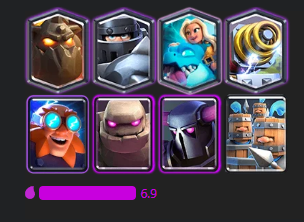
\includegraphics[width=0.6\textwidth]{images/DeckScarso.png}
\caption{Soluzione pessima, deck sbilanciato e troppo costoso (fitness = 188).}
\end{figure}

\begin{figure}[H]
\centering
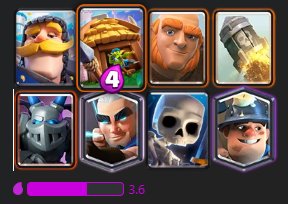
\includegraphics[width=0.6\textwidth]{images/DeckMigliore.png}
\caption{Soluzione buona, deck equilibrato e con costo moderato (fitness = 180).}
\end{figure}


\subsection{Funzione di fitness adottata}

La funzione di fitness adottata è una funzione non lineare basata su tre componenti principali:

\[
F(s) = Q_{\text{attacco}}(s) + Q_{\text{difesa}}(s) - P_{\text{bilanciamento}}(s)
\]

dove:
\begin{itemize}
    \item $Q_{\text{attacco}}(s)$ misura la qualità offensiva del deck,
    \item $Q_{\text{difesa}}(s)$ misura la qualità difensiva del deck,
    \item $P_{\text{bilanciamento}}(s)$ rappresenta una penalità per configurazioni sbilanciate.
\end{itemize}

La scelta che ha portato alla creazione di questa funzione di fitness, è stata quella di basarsi sulla conoscenza del dominio applicativo degli sviluppatori.

Inoltre la funzione di fitness definita in questo capitolo viene utilizzata come criterio di valutazione all’interno degli algoritmi di ricerca e ottimizzazione descritti nel capitolo successivo.

\subsection{Qualità di attacco e difesa}

La qualità offensiva è definita come:

\[
Q_{\text{attacco}} = \sqrt{\text{DannoMedio}} \cdot (1 + 0.2 \cdot \text{NumeroTorre}) \cdot (1 + 0.2 \cdot \text{VelocitàMedia})
\]

La qualità difensiva è definita come:

\[
Q_{\text{difesa}} = \sqrt{\frac{\text{VitaMedia}}{6}} \cdot (1 + 0.1 \cdot \text{NumeroPortata}) \cdot (1 + 0.05 \cdot \text{EffettiAggiuntivi})
\]

L’utilizzo della radice quadrata sulle variabili principali (\textit{DannoMedio} e \textit{VitaMedia}) consente di ridurre l’influenza delle feature con dominio numerico elevato, introducendo una normalizzazione non lineare che limita l’effetto di valori estremi e migliora la stabilità della funzione di fitness.

\medskip
Il dominio dei valori di \textit{DannoMedio} e \textit{VitaMedia} è significativamente differente, come mostrato nella \textit{Figura 3}. 
Per garantire un bilanciamento equilibrato tra le due variabili, la variabile \textit{VitaMedia} viene normalizzata sostituendola con:

\[
\frac{\text{VitaMedia}}{6}
\]

\begin{figure}[H]
\centering

\includegraphics[width=0.7\textwidth]{images/grafico1.png}
\label{grafico1}
\caption{Distribuzione dei valori di DannoMedio e VitaMedia}
\end{figure}

\begin{figure}[H]
\centering
\caption{Distribuzione normalizzata dei valori di VitaMedia}

\includegraphics[width=0.7\textwidth]{images/grafico2.png}
\end{figure}

\subsubsection{Scelta delle variabili per le componenti $Q_{\text{attacco}}$ e $Q_{\text{difesa}}$}

Le variabili utilizzate per le componenti $Q_{\text{attacco}}$ e $Q_{\text{difesa}}$ sono state selezionate sulla base della conoscenza del dominio di Clash Royale e dell’analisi delle caratteristiche strategicamente rilevanti per la valutazione di un deck.

\paragraph{Variabili per $Q_{\text{attacco}}:$}
La componente offensiva è modellata tramite le seguenti variabili:

\begin{itemize}
    \item \textit{DannoMedio}: rappresenta il danno medio al secondo delle carte del deck ed è la principale misura della capacità offensiva.
    \item \textit{NumeroTorre}: indica il numero di carte il cui bersaglio principale è la torre, modellando la presenza di win condition e la capacità di infliggere danni diretti alle strutture avversarie.
    \item \textit{VelocitàMedia}: rappresenta la velocità media delle truppe nel deck ed è utilizzata per modellare la pressione offensiva e la rapidità di esecuzione delle strategie di attacco.
\end{itemize}

\paragraph{Variabili per $Q_{\text{difesa}}:$}
La componente difensiva è modellata tramite le seguenti variabili:

\begin{itemize}
    \item \textit{VitaMedia}: rappresenta la quantità media di punti vita delle truppe e degli edifici nel deck ed è una misura della capacità di resistenza difensiva.
    \item \textit{NumeroPortata}: indica il numero di carte in grado di colpire unità sia volanti che terrestri, modellando la capacità di controllo del campo di battaglia.
    \item \textit{EffettiAggiuntivi}: rappresenta un punteggio aggregato degli effetti speciali delle carte (ad esempio congelamento, rallentamento, generazione di truppe e danni ad area), che contribuiscono al controllo e alla gestione delle minacce avversarie.
\end{itemize}

\subsubsection{Scelta dei parametri per le componenti $Q_{\text{attacco}}$ e $Q_{\text{difesa}}$}

I parametri numerici utilizzati nelle componenti $Q_{\text{attacco}}$ e $Q_{\text{difesa}}$ sono stati selezionati sulla base di un euristica empirica data dalla  conoscenza del dominio e da una fase preliminare di sperimentazione.

In particolare, i coefficienti moltiplicativi associati alle variabili \textit{NumeroTorre}, \textit{VelocitàMedia}, \textit{NumeroPortata} ed \textit{EffettiAggiuntivi} (sono rispettivamente 0.2, 0.2, 0.1 e 0.05) 

\subsection{Penalità di bilanciamento}

La penalità per il bilanciamento del deck è definita come:

\[
P_{\text{bilanciamento}} = p_{\text{costo}} + p_{\text{bersaglio}} + p_{\text{volante}} + p_{\text{portata}} + p_{\text{incantesimi}} + p_{\text{edifici}}
\]

Le singole penalità sono definite come segue:

\[
p_{\text{costo}} = (\text{CostoMedio} - 1)^3
\]

\[
p_{\text{bersaglio}} =
\begin{cases}
3 \cdot \text{NumeroTorre} & \text{se } \text{NumeroTorre} > 2 \\
0 & \text{altrimenti}
\end{cases}
\]

\[
p_{\text{portata}} =
\begin{cases}
15 & \text{se } \text{NumeroPortata} = 0 \\
0 & \text{altrimenti}
\end{cases}
\]

\[
p_{\text{incantesimi}} =
\begin{cases}
12 & \text{se } \text{NumeroIncantesimi} = 0 \\
0 & \text{altrimenti}
\end{cases}
\]

\[
p_{\text{volante}} =
\begin{cases}
10 & \text{se } \text{NumeroVolanti} = 0 \\
4 & \text{se } \text{NumeroVolanti} > 3 \\
0 & \text{altrimenti}
\end{cases}
\]

\[
p_{\text{edifici}} =
\begin{cases}
5 & \text{se } \text{NumeroEdifici} = 0 \\
12 & \text{se } \text{NumeroEdifici} > 2 \\
0 & \text{altrimenti}
\end{cases}
\]

\subsubsection{Scelta delle variabili per la componente $P_{\text{bilanciamento}}$}

Le variabili utilizzate nella componente di penalità $P_{\text{bilanciamento}}$ sono state selezionate sulla base della conoscenza del dominio di Clash Royale e rappresentano alcune delle caratteristiche strategicamente più rilevanti nella costruzione di un deck efficace.

In particolare, tali variabili riflettono aspetti fondamentali del gioco, come il costo medio in elisir, la capacità di attaccare la torre, la copertura aerea, la possibilità di colpire unità volanti, la presenza di incantesimi e il supporto difensivo fornito dagli edifici. 
La scelta di queste variabili consente di penalizzare configurazioni fortemente sbilanciate che, pur presentando buone statistiche di attacco o difesa, risultano poco utilizzabili in una reale partita di gioco.

Di seguito vengono descritte le singole variabili che contribuiscono alla penalità di bilanciamento.

\paragraph{Costo:}
Il costo medio in elisir rappresenta uno degli aspetti più critici nella costruzione di un deck. 
Deck con costo medio troppo elevato risultano lenti e difficili da gestire durante una partita, penalizzando la capacità di risposta dell’utente. 
Per questo motivo, la variabile $p_{\text{costo}}$ introduce una penalità crescente al crescere del costo medio del deck.
Per la formula la decisione è stata quella di un elevazione al cubo, per rendere il contributo della variabile più forte rispetto alle altre dato che è la più importante 

\paragraph{Bersaglio:}
La variabile relativa al numero di carte con bersaglio esclusivo sugli edifici e quindi come principale la torre, è utilizzata per evitare deck eccessivamente focalizzati sull’attacco diretto. 
Un numero elevato di tali carte riduce la capacità del deck di difendere efficacemente contro le truppe avversarie, rendendo la configurazione fragile dal punto di vista difensivo.

\paragraph{Volante:}
La presenza di truppe volanti è fondamentale per fronteggiare unità che non possono essere colpite da truppe terrestri, e per usare strategie di attacco più difficili da fronteggiare
L’assenza totale di truppe volanti, così come una loro presenza eccessiva, può generare forti squilibri. 
Per questo motivo, la penalità $p_{\text{volante}}$ agisce sia in caso di assenza sia in caso di eccesso di truppe volanti.

\paragraph{Incantesimi:}
Gli incantesimi svolgono un ruolo chiave nel controllo del campo di battaglia, consentendo di eliminare gruppi di truppe o supportare le proprie unità. 
Un deck privo di incantesimi risulta generalmente meno flessibile, motivo per cui l’assenza totale di carte di questo tipo è penalizzata.

\paragraph{Edifici:}
Le carte di tipologia edificio forniscono supporto difensivo e controllo del campo. 
L’assenza di edifici riduce la capacità del deck di gestire unità avversarie pesanti, mentre un numero eccessivo di edifici limita le opzioni offensive. 
La penalità $p_{\text{edifici}}$ è quindi applicata sia sull'assenza di questi che su un numero eccessivo nel deck 

\subsubsection{Scelta dei parametri della funzione di penalità}

I parametri numerici utilizzati nella componente $P_{\text{bilanciamento}}$ non derivano da un modello teorico formale, ma sono stati determinati tramite un processo di euristica empirica basato sulla conoscenza del dominio di Clash Royale da parte degli sviluppatori.

In particolare, i valori assegnati alle singole penalità sono il risultato di considerazioni qualitative sulle dinamiche di gioco e di sperimentazioni preliminari volte a individuare configurazioni di deck realistiche ed efficaci. 
L’obiettivo principale nella scelta di tali parametri è stato quello di penalizzare in modo significativo le situazioni considerate critiche dal punto di vista strategico, senza tuttavia annullare completamente il contributo positivo delle componenti di attacco e difesa.

\subsection{Limiti della funzione di fitness}

La funzione di fitness proposta rappresenta una semplificazione del dominio di Clash Royale e non modella esplicitamente le sinergie tra carte né il meta-game competitivo.
Inoltre, la valutazione è indipendente dall’avversario e dal contesto di partita, assumendo che la qualità del deck possa essere stimata in modo isolato.


\section{Scelte tecniche progettuali: definizione degli algoritmi}

\subsection{Inquadramento del problema}

Il problema della generazione automatica di deck di Clash Royale è riconducibile a un problema di ottimizzazione combinatoria caratterizzato da uno spazio degli stati estremamente ampio e dalla presenza di numerosi vincoli.
In tale contesto, l’utilizzo di algoritmi di ricerca esatta risulta impraticabile, rendendo necessario l’impiego di tecniche di ricerca approssimata e metaeuristiche.

Gli algoritmi selezionati per questo progetto sono stati scelti con l’obiettivo di esplorare efficacemente lo spazio delle soluzioni e individuare configurazioni di elevata qualità in tempi computazionali bassi.


\subsection{Algoritmi considerati}

Nel contesto del progetto \textit{Deck-BuilderCR} sono stati presi in considerazione principalmente due approcci:
\begin{itemize}
    \item L'utilizzo dell'algoritmo \textit{Hill Climbing} è stata la scelta iniziale, ma in secondo momento scartata per delle profonde lacune verso il dominio applicativo 
    \item L'utilizzo di un \textit{Algoritmo Genetico} è stata la solzuione finale presa in considerazione dopo aver scartato la soluzione che prevedeva l'algoritmo Hill Climbing 
\end{itemize}

\subsection{Hill Climbing}

L’algoritmo di \textit{Hill Climbing} è uno dei più semplici algoritmi di ricerca locale e ha l’obiettivo di migliorare iterativamente una soluzione corrente esplorando il suo intorno nello spazio di ricerca, fino al raggiungimento di un massimo (o minimo) locale della funzione di fitness.

Nonostante la sua semplicità, l’Hill Climbing è stato inizialmente considerato una possibile soluzione per il problema affrontato, in quanto il dominio non presenta un vero e proprio ottimo globale assoluto. 
Infatti, nel contesto di Clash Royale, la qualità di un deck non è determinata unicamente da criteri oggettivi, ma dipende anche da preferenze soggettive dei giocatori e da stili di gioco differenti.

Tuttavia, come verrà discusso nelle sezioni successive, l’approccio basato su Hill Climbing presenta limitazioni significative nel dominio considerato, che ne hanno motivato lo scarto come soluzione finale.

\subsubsection{Struttura dei vicini}

La struttura dei vicini è definita tramite una funzione:

\[
N : \mathcal{S} \rightarrow \mathcal{P}(\mathcal{S})
\]

dove:
\begin{itemize}
    \item $\mathcal{S}$ rappresenta l’insieme di tutte le soluzioni possibili, ovvero l’insieme di tutti i deck creabili a partire dalle carte disponibili;
    \item $\mathcal{P}(\mathcal{S})$ indica l’insieme delle parti di $\mathcal{S}$;
    \item $N(s) \subseteq \mathcal{S}$ è l’insieme delle soluzioni vicine allo stato $s$.
\end{itemize}

Nel contesto del progetto, due soluzioni sono considerate vicine se differiscono per una singola carta. 
In particolare, una soluzione vicina è ottenuta sostituendo una delle 8 carte del deck corrente con una carta diversa selezionata dall’insieme delle carte disponibili.

Assumendo la presenza di 113 carte totali e l’assenza di duplicati, ogni stato presenta fino a $8 \times 105 = 840$ soluzioni vicine possibili.

\subsubsection{Condizioni di arresto}

Nel progetto, l’algoritmo di Hill Climbing termina in una delle seguenti condizioni:

\begin{enumerate}
    \item non esiste una soluzione vicina con valore di fitness maggiore rispetto alla soluzione corrente:
    \[
    \nexists s' \in N(s) \; : \; f(s') > f(s)
    \]
    \item viene raggiunto un numero massimo prefissato di iterazioni pari a 300.
\end{enumerate}

La seconda condizione è stata introdotta per evitare che l’algoritmo impieghi un tempo eccessivo nel tentativo di migliorare una soluzione che non presenta ulteriori miglioramenti significativi.

Il valore massimo di 300 iterazioni è stato determinato empiricamente a seguito di test sperimentali con valori inferiori e superiori. 
Tale scelta rappresenta un compromesso (\textit{trade-off}) tra efficienza computazionale e qualità della soluzione ottenuta.

\subsubsection{Motivazioni dello scarto dell’algoritmo Hill Climbing}

Nonostante la semplicità implementativa e le soluzioni con alta fitness che dava, l’algoritmo di Hill Climbing si è rivelato non adeguato al dominio applicativo considerato.

In particolare, il problema della generazione di deck di Clash Royale presenta uno spazio delle soluzioni altamente multimodale, caratterizzato dalla presenza di numerosi ottimi locali; inoltre come  fattore più importante, abbiamo che il problema della generazione di un deck di Clash Royale non ha una soluzione ottima globale deinitiva, ma ci sono varie soluzioni ottime in base anche alle preferenze soggettive del giocatore.
In tale contesto, l’Hill Climbing tende a convergere rapidamente verso soluzioni localmente ottimali, senza la capacità di esplorare regioni alternative dello spazio di ricerca.

Inoltre, l’algoritmo non garantisce un’adeguata diversità delle soluzioni generate, producendo spesso deck molto simili tra loro, se non addirittura quasi sempre uguali e limitando la possibilità di individuare configurazioni significativamente differenti ma potenzialmente più efficaci.

Queste limitazioni hanno portato allo scarto dell’Hill Climbing come strategia principale, rendendo necessario l’utilizzo di un approccio in grado di bilanciare efficacemente esplorazione e sfruttamento dello spazio delle soluzioni, producendo quasi sempre soluzioni diverse che possano soddisfare 

\subsection{Algoritmo Genetico}

A seguito dello scarto dell’algoritmo di Hill Climbing, è stato adottato come soluzione finale un approccio basato sulla famiglia degli \textit{Algoritmi Genetici}. 
Tale scelta è motivata dalla necessità di esplorare in modo più efficace uno spazio delle soluzioni ampio, complesso e fortemente multimodale, riducendo il rischio di convergenza prematura verso ottimi locali.

L’Algoritmo Genetico consente infatti di mantenere una popolazione di soluzioni candidate e di introdurre diversità nel processo di ricerca tramite operatori stocastici, risultando particolarmente adatto al dominio applicativo considerato

\subsubsection{Rappresentazione degli individui}

Ogni individuo della popolazione rappresenta una possibile soluzione del problema ed è modellato come un vettore di geni di lunghezza fissa pari a 8:

\[
I = (g_1, g_2, \dots, g_8)
\]

dove ciascun gene $g_i$ rappresenta una carta del deck.

Il dominio dei geni è costituito dall’insieme delle carte disponibili nel gioco, escludendo i Campioni, in accordo con le assunzioni e le limitazioni del dominio definite nel Capitolo~1.

\subsubsection{Inizializzazione della popolazione}

La popolazione iniziale è generata in modo completamente casuale, con una dimensione pari a 100 individui. 
Durante la fase di inizializzazione, possono essere applicati eventuali vincoli imposti dall’utente, come la presenza obbligatoria di alcune carte nel deck.

La dimensione del \textit{mating pool} invece è leggermente inferiore, ed è 80, garantendo che quasi tutti gli individui possano partecipare al processo di crossover.

La scelta di un’inizializzazione casuale è motivata dalle caratteristiche del dominio di Clash Royale, nel quale esistono deck efficaci basati su combinazioni molto differenti di carte. 
Un approccio casuale consente quindi di introdurre fin dall’inizio una buona diversità nella popolazione.
Mentre la scelta di una size popolation di 100 e di un mating pool di 80, è stata presa dopo varie sperimentazioni che hanno portato alla conclusione che è meglio avere una dimensione di possibili soluzioni abbastanza ampia ma non troppo, per avere un giusto bilanciamento tra efficenza della solzuione finale e costo computazionale
\subsubsection{Operatore di selezione}

Come operatore di selezione è stato adottato il metodo di \textit{Rank Selection}. 
In questo approccio, gli individui vengono ordinati in base al valore di fitness e la probabilità di selezione dipende dalla posizione in classifica piuttosto che dal valore assoluto della fitness.

Questa scelta consente di ridurre la pressione selettiva e di preservare la diversità della popolazione, favorendo una migliore esplorazione dello spazio delle soluzioni, a fronte di un lieve aumento del costo computazionale dovuto all’ordinamento (\textit{trade-off}).

\subsubsection{Operatore di crossover}

L’operatore di crossover scelto è il \textit{Uniform Crossover}. 
Durante il crossover, ciascun gene del figlio viene selezionato casualmente da uno dei due genitori.

Nel caso in cui il deck generato risulti non valido, l’operazione di crossover viene ripetuta per un numero massimo prefissato di tentativi. 
Se anche dopo tali tentativi il figlio risulta invalido, viene restituito uno dei due genitori selezionato casualmente.

La probabilità di crossover è fissata pari a 1, in modo da favorire una costante ricombinazione genetica e una migliore esplorazione dello spazio degli stati. 
Nel raro caso in cui il crossover non venga applicato, l’individuo restituito è uno dei due genitori scelto casualmente.

\subsubsection{Operatore di mutazione}

Come operatore di mutazione è stato adottato il \textit{Random Resetting}. 
In questo approccio, un gene viene selezionato casualmente e sostituito con un’altra carta disponibile, in modo tale da non violare i vincoli di validità del deck.

La probabilità di mutazione è fissata a 0.8
La scelta di avere una probabilità di mutazione cosi alta consente di avere molta casualità, che per il dominio del problema è fondamentale 

\section{Interfaccia Grafica}

L’interfaccia grafica sviluppata ha lo scopo di facilitare l’interazione dell’utente con il progetto nel suo complesso.  
Attraverso il menù principale è possibile selezionare il tipo di algoritmo da utilizzare, scegliendo tra Hill Climbing e Algoritmo Genetico, e configurarne i rispettivi parametri, permettendo così all’utente di personalizzare l’esecuzione dell’algoritmo.

Inoltre, l’interfaccia consente di selezionare fino a quattro carte iniziali che il mazzo finale dovrà obbligatoriamente contenere, vincolando in questo modo il processo di generazione del deck.

Nella schermata principale vengono mostrati i risultati finali dell’esecuzione, includendo la fitness ottenuta e le principali statistiche relative alle carte del mazzo generato, calcolate in base ai parametri selezionati dall’utente.  
È inoltre presente una sezione dedicata allo storico delle esecuzioni, nella quale sono memorizzate tutte le generazioni prodotte dall’algoritmo, consentendo all’utente di consultarle in qualsiasi momento.

\subsection{Configurazione per l’utente finale}

Per eseguire correttamente l’applicazione e avviare l’interfaccia grafica, è necessario seguire i passaggi descritti di seguito, utilizzando il terminale dell’IDE (in questo caso PyCharm).

\begin{enumerate}
    \item \textbf{Installazione delle dipendenze} (sia su macOS che su Windows):
    \begin{verbatim}
    pip install -r requirements.txt
    \end{verbatim}

    \item \textbf{Inizializzazione dell’ambiente virtuale}:
    
    \textit{Su macOS}:
    \begin{verbatim}
    source .venv/bin/activate
    \end{verbatim}

    \textit{Su Windows}:
    \begin{verbatim}
    .venv\Scripts\activate
    \end{verbatim}

    \item \textbf{Avvio dell’interfaccia grafica}:
    \begin{verbatim}
    streamlit run DeckBuilderCR/GUI/guiClashRoyale.py
    \end{verbatim}
\end{enumerate}

\section{Risultati e conclusione}

I risultati presentati in questo capitolo sono stati ottenuti eseguendo sia l’algoritmo genetico sia l’algoritmo di Hill Climbing per un totale di 50 esecuzioni indipendenti ciascuno.  
I parametri utilizzati per l’algoritmo genetico durante le fasi di test sono quelli descritti nel Capitolo~4.4.

\subsection{Fitness media}

L’analisi dei risultati mostra che l’algoritmo di Hill Climbing ottiene, in media, soluzioni con una fitness più elevata rispetto all’algoritmo genetico.  
In particolare, il GA produce mazzi con una fitness media pari a 47{,}3, mentre l’Hill Climbing raggiunge una fitness media di 57{,}9.

Questo risultato indica che, dal punto di vista puramente ottimizzativo, l’Hill Climbing tende a convergere verso soluzioni di qualità superiore. Tuttavia, tale comportamento deve essere valutato in relazione alle altre metriche considerate e agli obiettivi complessivi del problema.

\subsection{Velocità di esecuzione}

Per quanto riguarda le prestazioni temporali, l’algoritmo genetico risulta significativamente più rapido rispetto all’Hill Climbing.  
Il tempo medio di esecuzione dell’Hill Climbing è pari a 4535 ms per singola esecuzione, mentre l’algoritmo genetico impiega in media soltanto 125 ms.

Questo divario è dovuto alla natura iterativa e locale dell’Hill Climbing, che richiede numerosi passi di miglioramento successivo, a fronte di un GA che sfrutta operatori evolutivi in grado di esplorare lo spazio delle soluzioni in modo più efficiente dal punto di vista computazionale.

\subsection{Varianza dei risultati}

La varianza rappresenta una misura della dispersione dei risultati attorno al valore medio e fornisce indicazioni sulla stabilità e sulla diversità delle soluzioni generate.

Formalmente, data una serie di valori di fitness ottenuti da $N$ esecuzioni indipendenti dell’algoritmo,
\[
f_1, f_2, \dots, f_N,
\]
la varianza è definita come:
\[
\sigma^2 = \frac{1}{N} \sum_{i=1}^{N} (f_i - \bar{f})^2
\]
dove $\bar{f}$ rappresenta la fitness media, calcolata come:
\[
\bar{f} = \frac{1}{N} \sum_{i=1}^{N} f_i.
\]

Nel nostro caso, l’algoritmo genetico presenta una varianza pari a 5{,}99, mentre l’Hill Climbing mostra una varianza prossima allo zero.  
Sebbene una varianza bassa sia spesso considerata un indicatore positivo di stabilità, nel contesto specifico del problema tale comportamento risulta limitante.

Una varianza prossima allo zero indica infatti che, indipendentemente dallo stato iniziale, l’Hill Climbing converge quasi sempre verso soluzioni molto simili tra loro, suggerendo una forte dipendenza dai massimi locali dello spazio degli stati.  
Al contrario, la varianza osservata nel GA, pur rimanendo contenuta, è sufficientemente elevata da indicare la produzione di soluzioni diverse tra loro, caratteristica desiderabile nel problema in esame.

\subsection{Conclusione}

Sulla base delle analisi effettuate, la soluzione finale adottata è l’algoritmo genetico.  
Come anticipato nel Capitolo~2, il GA risulta maggiormente coerente con gli obiettivi del problema, grazie alla sua maggiore flessibilità e alla capacità di esplorare in modo più efficace lo spazio degli stati.

Sebbene l’Hill Climbing produca soluzioni mediamente più ottime in termini di fitness, esso soffre di una forte convergenza verso soluzioni simili, riducendo la varietà dei mazzi generati.  
L’algoritmo genetico, invece, pur non garantendo sempre la soluzione ottima, è in grado di generare soluzioni costantemente buone e sufficientemente diverse tra loro, rendendolo più adatto al contesto applicativo considerato.

\section{Disponibilità del codice sorgente}

Il codice sorgente completo del progetto, comprensivo dell’implementazione degli algoritmi, dell’interfaccia grafica e dei file di configurazione, è disponibile pubblicamente al seguente indirizzo:

\begin{center}
\url{https://github.com/girgio/Deck-BuilderCR}
\end{center}




\end{document}
